\documentclass[a4paper]{article}
\usepackage{latexsym,amssymb,amsmath,amsbsy,amsopn,amstext,xcolor,multicol}
\usepackage{ctex,hyperref,graphicx,wrapfig,fancybox,listings}
\usepackage{pgf,pgfarrows,pgfnodes,pgfautomata,pgfheaps,pgfshade}
\usepackage[top=1in, bottom=1in, left=1.25in, right=1.25in]{geometry}
\graphicspath{{pic/}}
\title{\bf 中间人攻击实验}
\date{2017.11}
\author{计64~翁家翌~2016011446}
\begin{document}
\kaishu
\ttfamily
\maketitle
%\tableofcontents
%\newpage
\section{实验环境}
攻击者:Ubuntu 16.04.3 LTS

路由:小米路由(Openwrt内核)、手机热点

靶机:Ubuntu 16.04、Win10、Macbook Pro、iPhone、iPad、小米手机等
\section{实验原理}
\begin{enumerate}
	\item 使用scapy构造arp包,对网关和受害者发送欺骗信息,修改其arp缓存
	\item scapy脚本嗅探所有src/dst为靶机ip地址,并且含有IP层信息的包,将其修改src/dst之后转发
	\item 配置本机iptables,其中ip\_forward选项设置为1,并且转发53,80,443端口至本机8080端口,以便mitmproxy进行处理;将用脚本处理之后的包发送至原地址
\end{enumerate}

其中,攻击脚本为\uline{mitm.py},包含构造ARP报文、嗅探数据包的功能;修改http数据流的脚本为\uline{a.py},实现了将所有图片旋转$180^\circ$的功能
\section{实验现象}
\subsection{Ubuntu 16.04}
查看路由和靶机的arp缓存,发现修改成功

修改iptables配置,如图\ref{fig:iptables}所示:
\begin{figure}[htp]
\centering
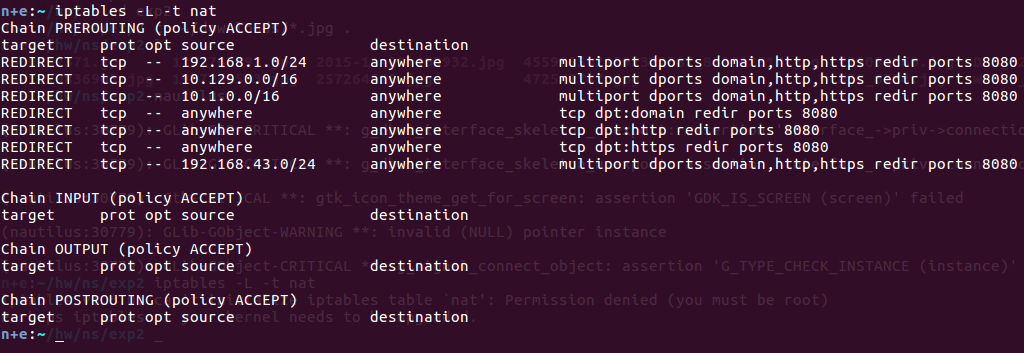
\includegraphics[width=0.89\linewidth]{iptables.png}
\caption{iptables的配置情况}
\label{fig:iptables}
\end{figure}

以root权限运行命令\uline{python3 mitm.py}和\uline{mitmproxy -T -s a.py},查看截获的流量,发现靶机成功被欺骗。(忘记截图了)

经过测试,虚拟机环境下的Ubuntu也能够被欺骗。
\subsection{Win10}
配置与之前相同。Win10被成功欺骗。在Win10上使用Chrome浏览器进行测试,效果如下:

\begin{figure}[htp]
\centering
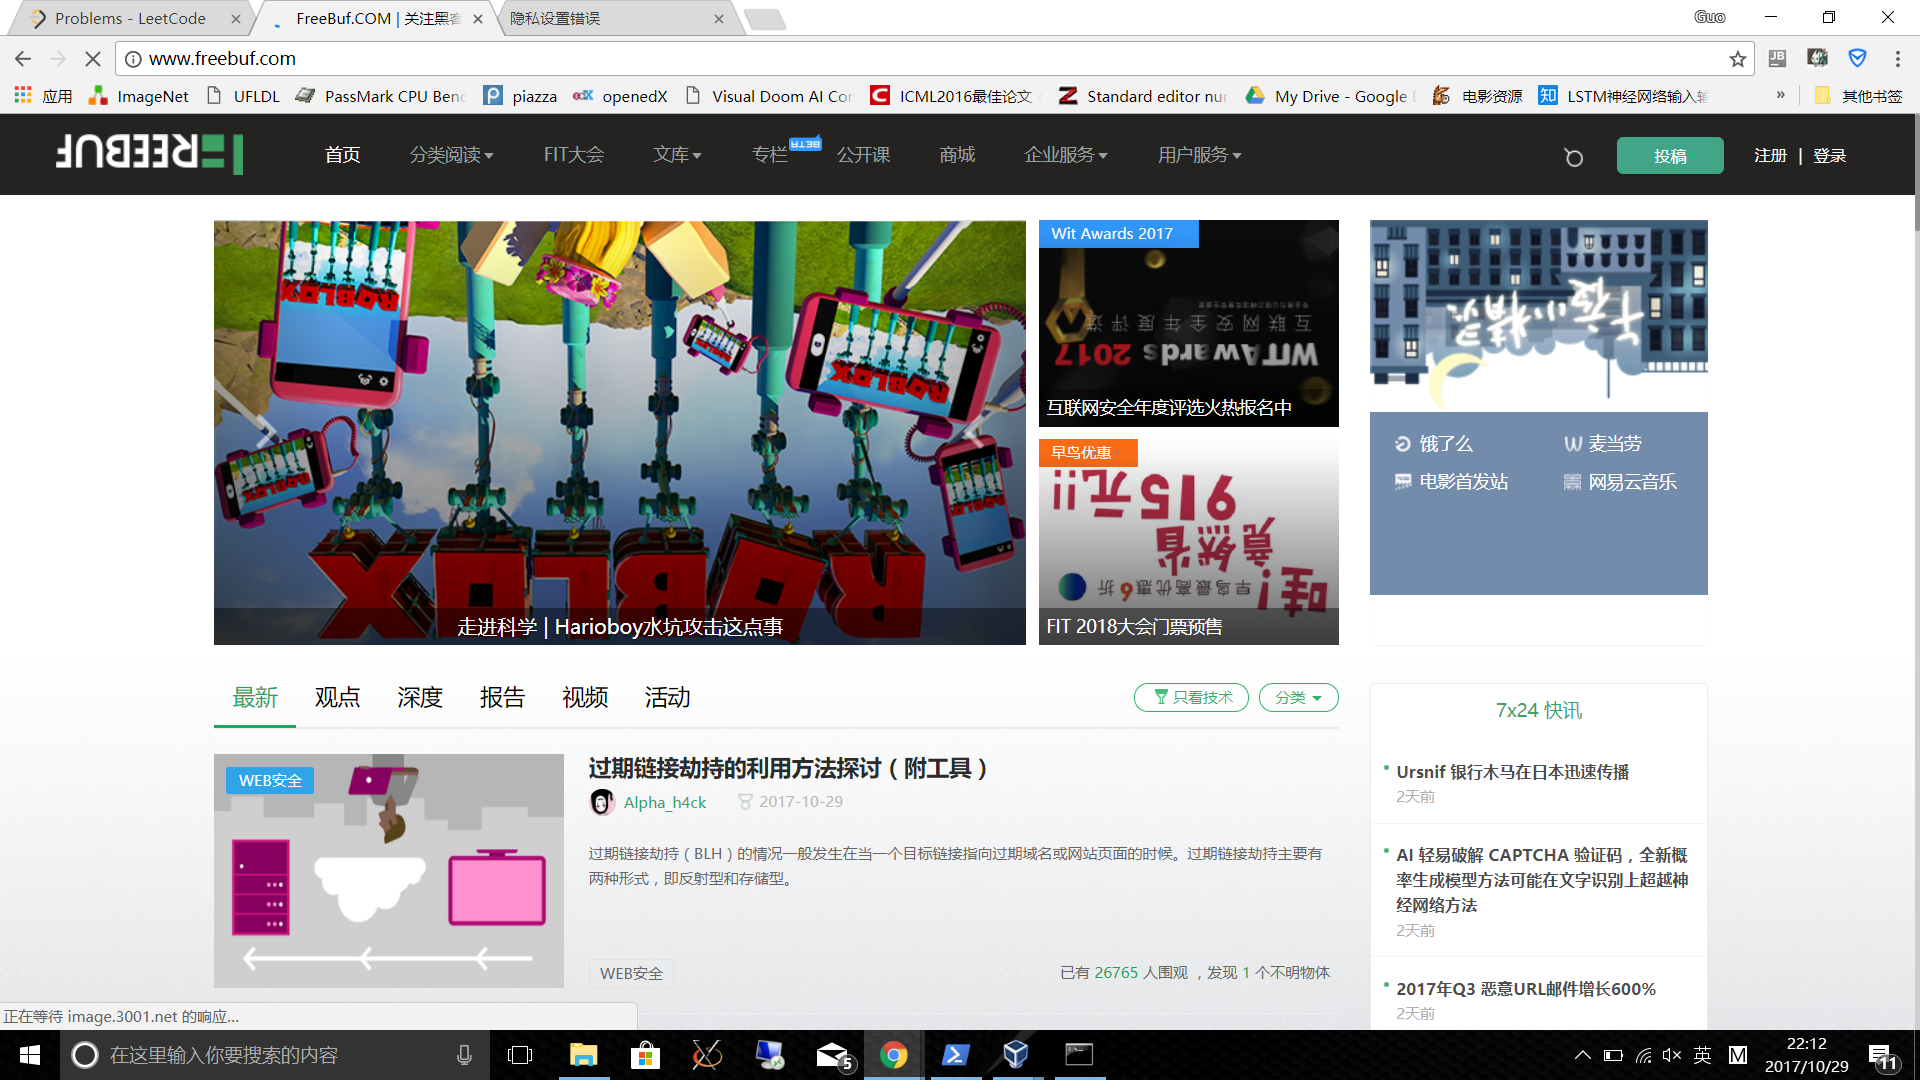
\includegraphics[width=0.9\linewidth]{freebuf.png}
\caption{访问\uline{http://www.freebuf.com}}
\label{fig:freebuf}
\end{figure}

图\ref{fig:freebuf}显示了靶机访问http网站的现象,可以看到访问正常,但是所有图片都被倒置了。在测试的时候,访问网页的速度较慢,可能是因为图片处理的速度不够快导致。

\begin{figure}[htp]
\centering
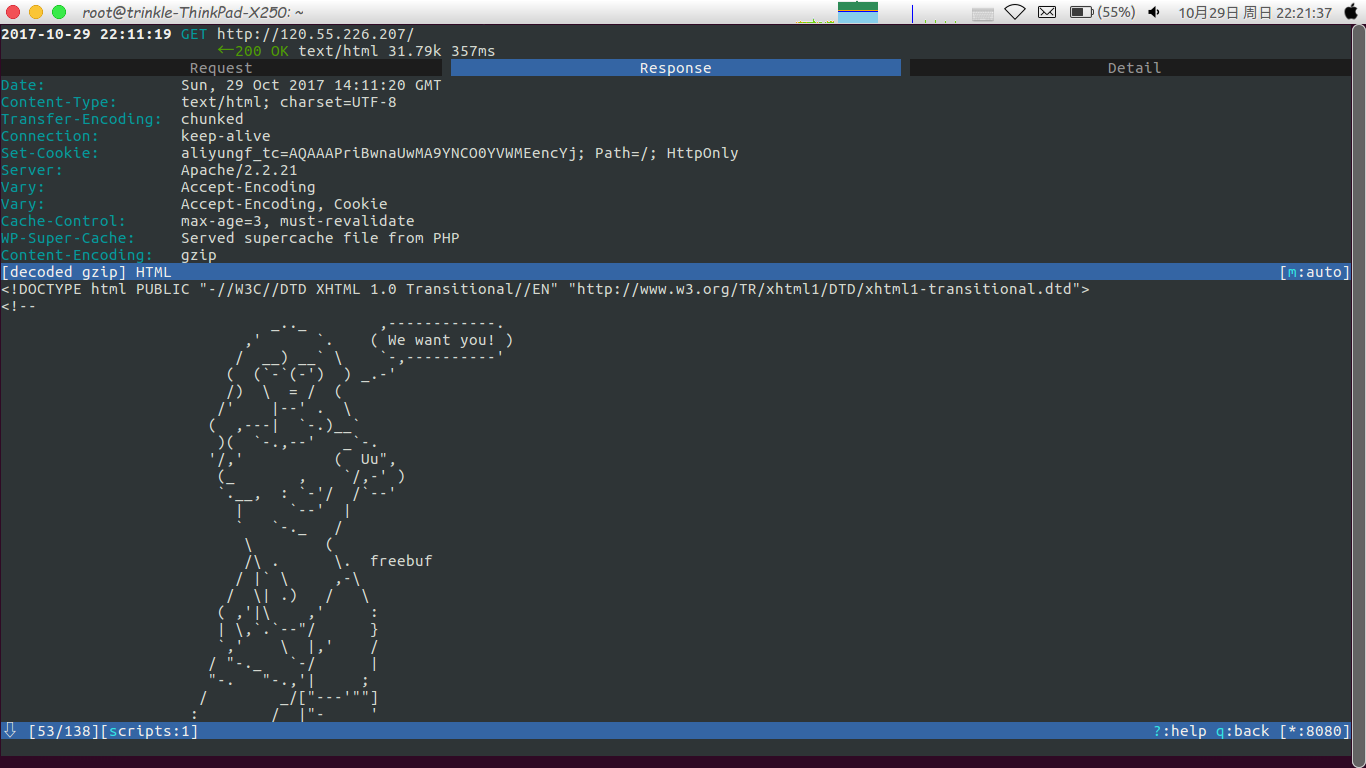
\includegraphics[width=0.9\linewidth]{request.png}
\caption{在攻击者上看到的http流量报文}
\label{fig:request}
\end{figure}

图\ref{fig:request}显示了攻击者机器上看到的http报文的数据。

\begin{figure}[htp]
\centering
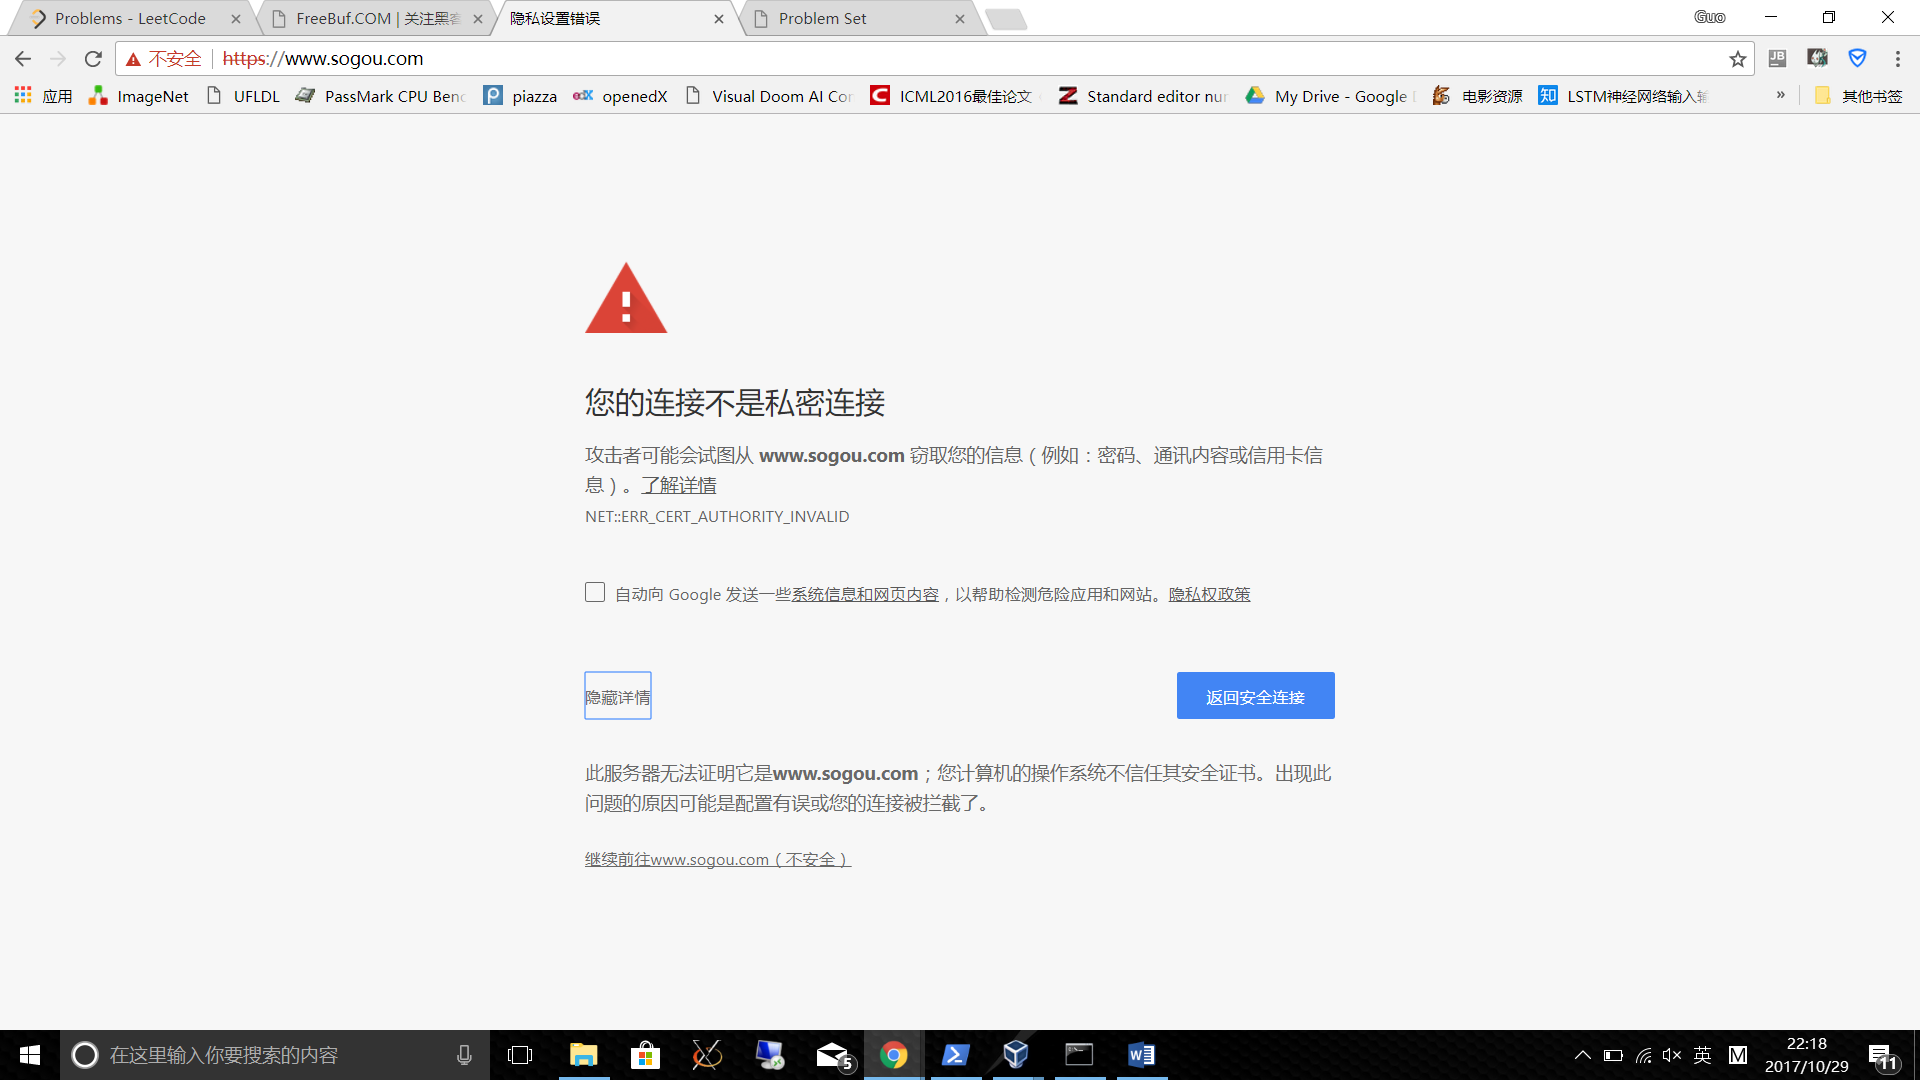
\includegraphics[width=0.9\linewidth]{error.png}
\caption{访问\uline{https://www.sogou.com}}
\label{fig:error}
\end{figure}

图\ref{fig:error}显示了靶机浏览器访问https网站的现象,可以看到浏览器提示链接不安全;但是如果点击最下面的超链接\uline{继续前往www.sogou.com(不安全)},就会出现目标网页,并且攻击者能够看到https的数据信息。

\begin{figure}[htp]
\centering
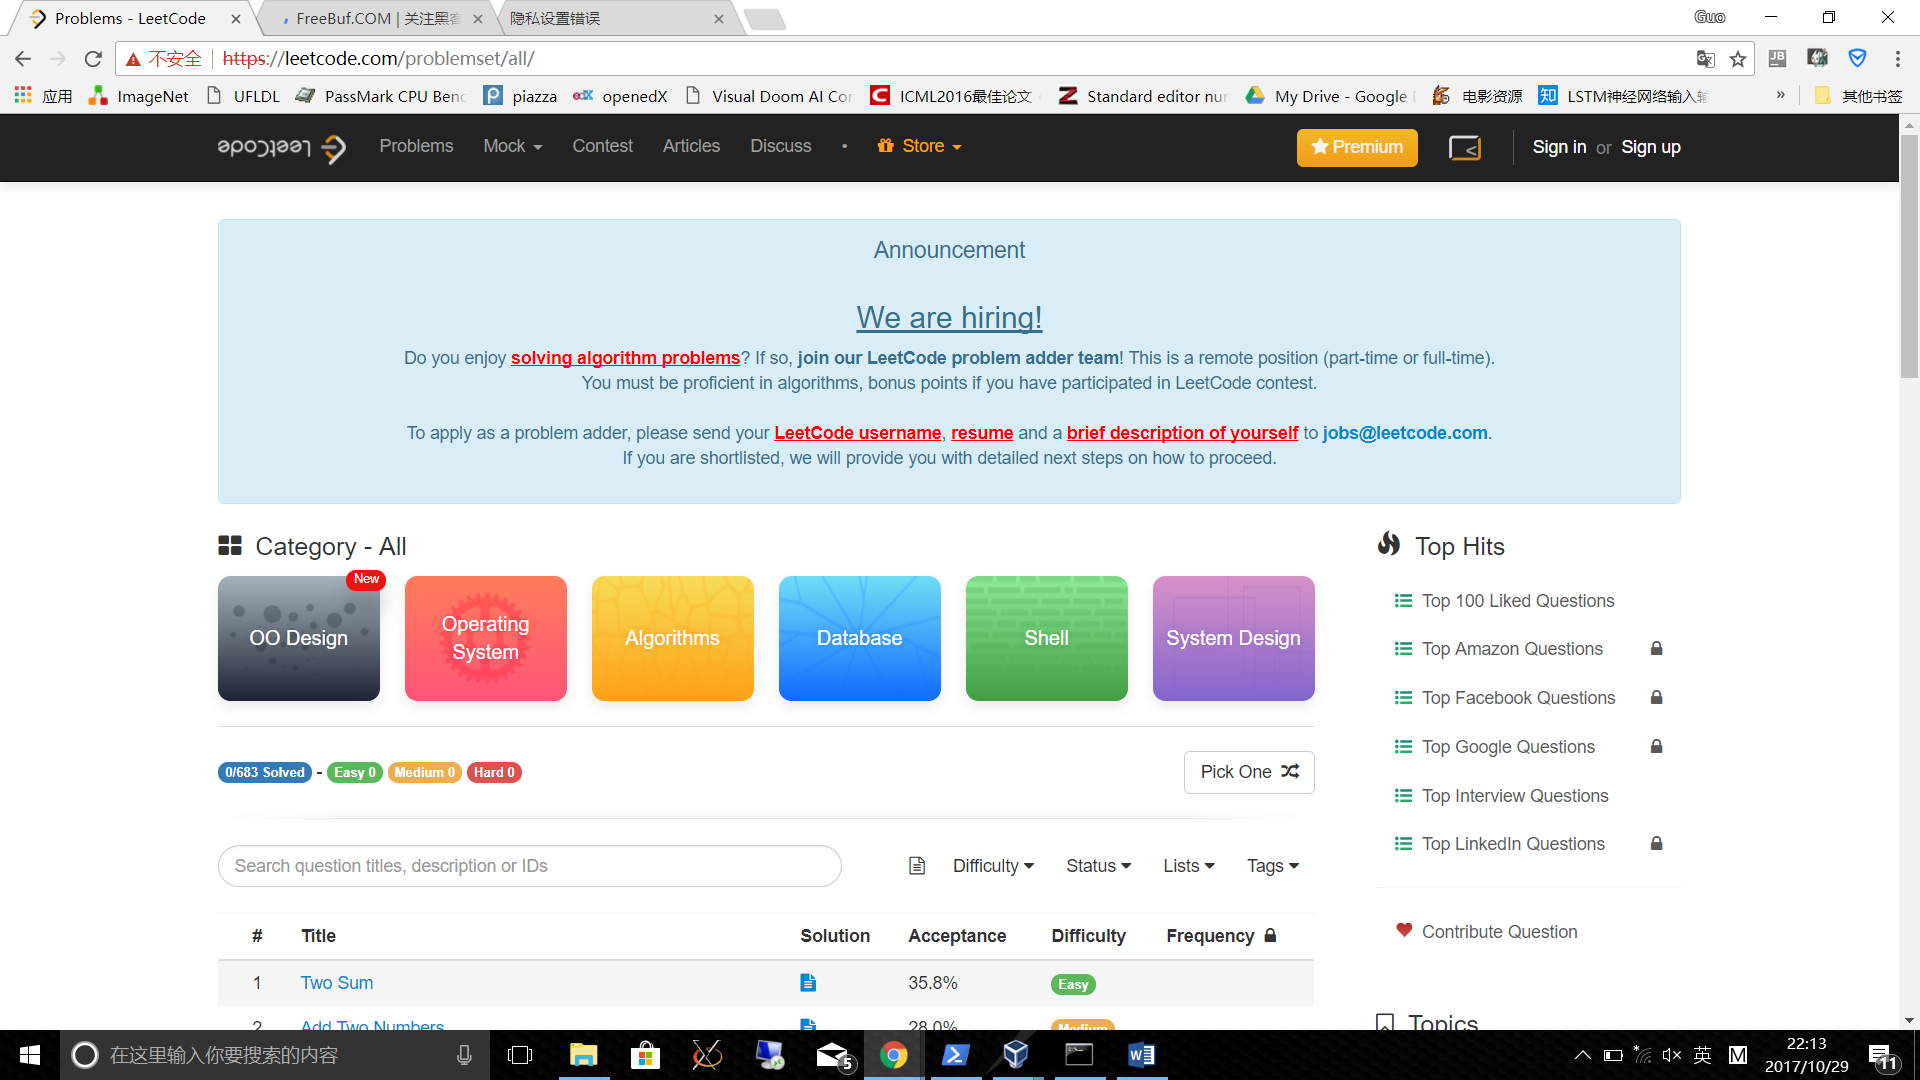
\includegraphics[width=0.9\linewidth]{leet.png}
\caption{访问\uline{https://leetcode.com}}
\label{fig:leetcode}
\end{figure}

图\ref{fig:leetcode}显示了靶机访问https网页,并且点击“继续前往”的选项之后的现象。可以看到在左上方的https被划了红线,并且里面的网页图片也被倒置(LeetCode的图标)。因此,看到如图\ref{fig:error}这种现象的网站,尽量不要选择不安全的访问方式,否则及有可能被中间人攻击。

\begin{figure}[htp]
\centering
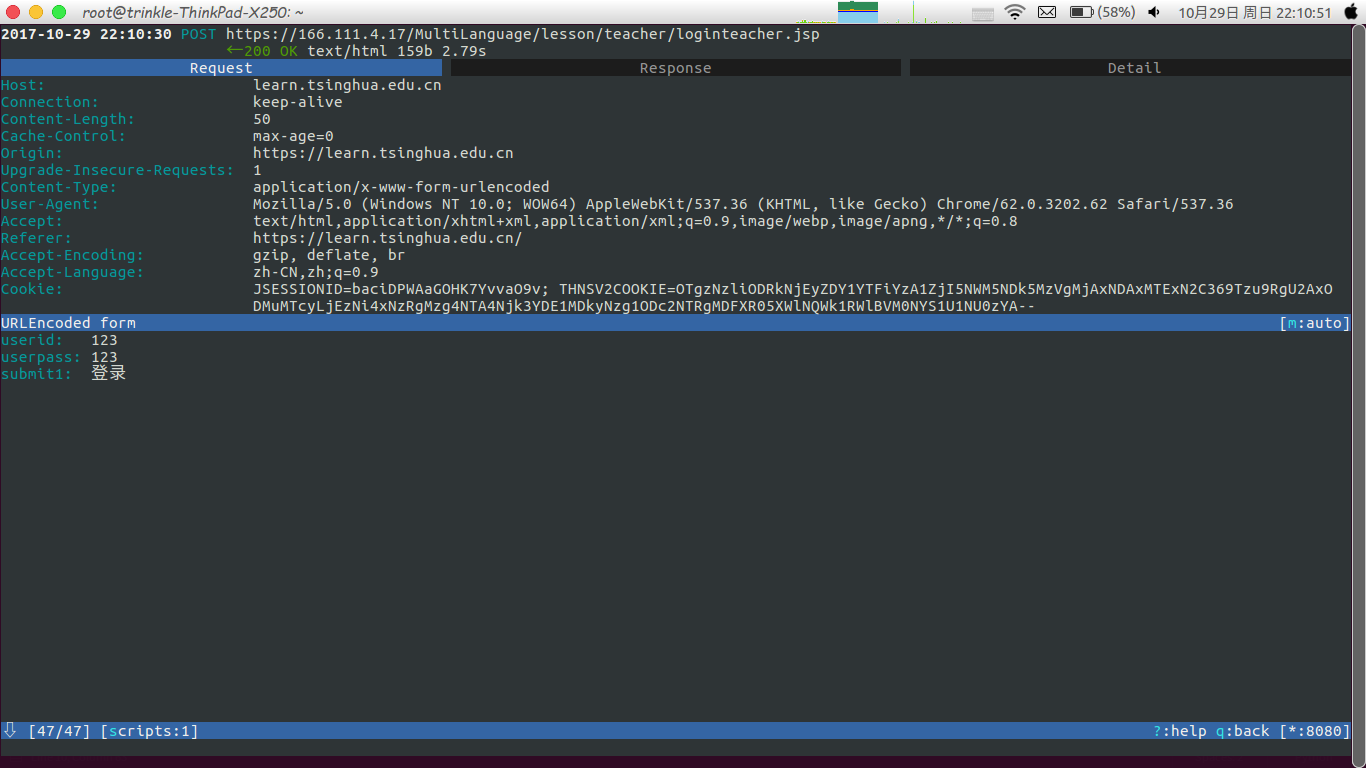
\includegraphics[width=0.9\linewidth]{wlxt.png}
\caption{登录网络学堂}
\label{fig:wlxt}
\end{figure}

图\ref{fig:wlxt}显示了靶机访问\uline{http://learn.tsinghua.edu.cn},并且随便敲了一个用户名和密码点击登录之后,在攻击者机器上看到的https报文。可以看到POST中URLEncoded form中的数据被一览无余。可见校园网的这些网站信息安全保护措施并不完美,应该全部使用https进行加密,而不是只在登录的时候使用https加密数据。

\subsection{Macbook Pro}
配置与之前相同。发现无法进行欺骗。

使用命令\uline{arp -n}查看arp缓存,发现arp缓存正常,未被修改。我猜想系统可能防arp毒化攻击。
\subsection{iPad/iPhone}
配置与之前相同。发现欺骗有时成功,有时不成功。可能是设备问题?

\begin{figure}[htp]
\centering
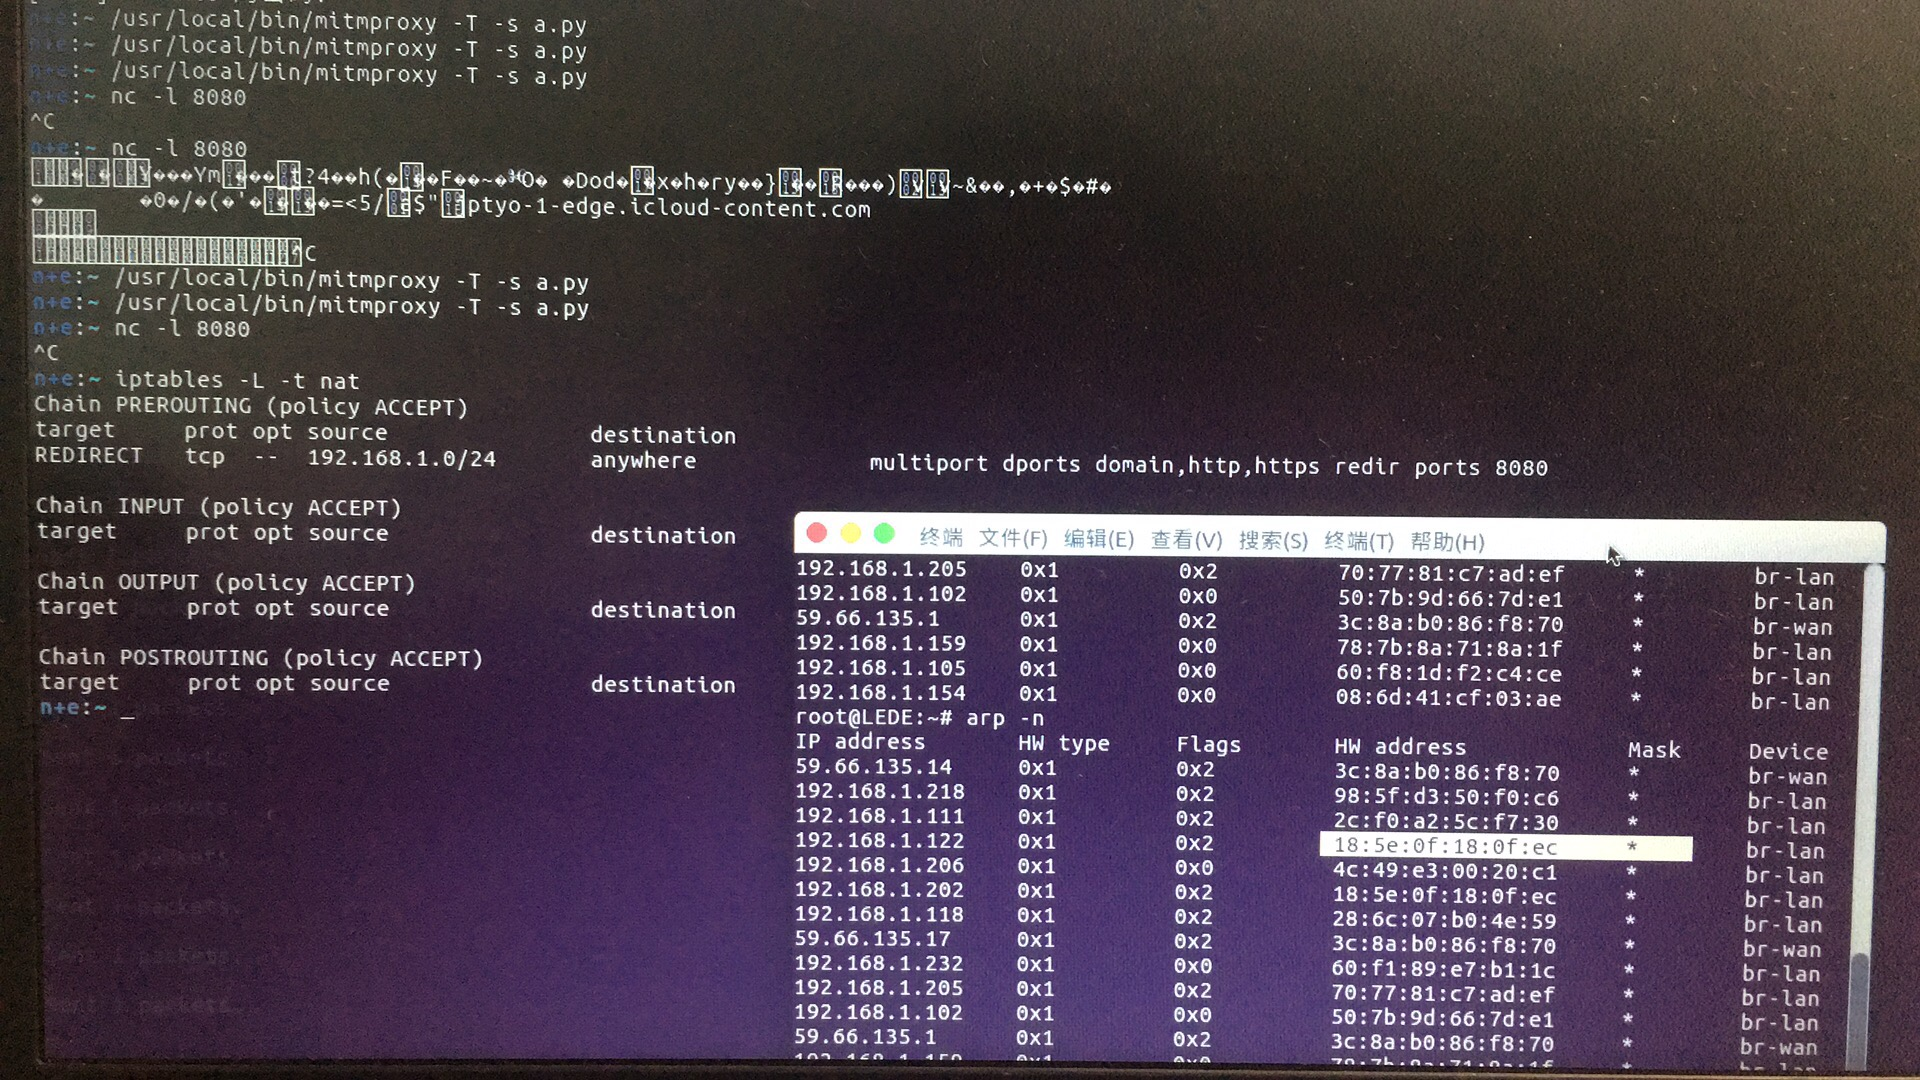
\includegraphics[width=0.9\linewidth]{wifi_arp.jpg}
\caption{路由器的arp缓存}
\label{fig:wifi_arp}
\end{figure}

\begin{figure}[htp]
\centering
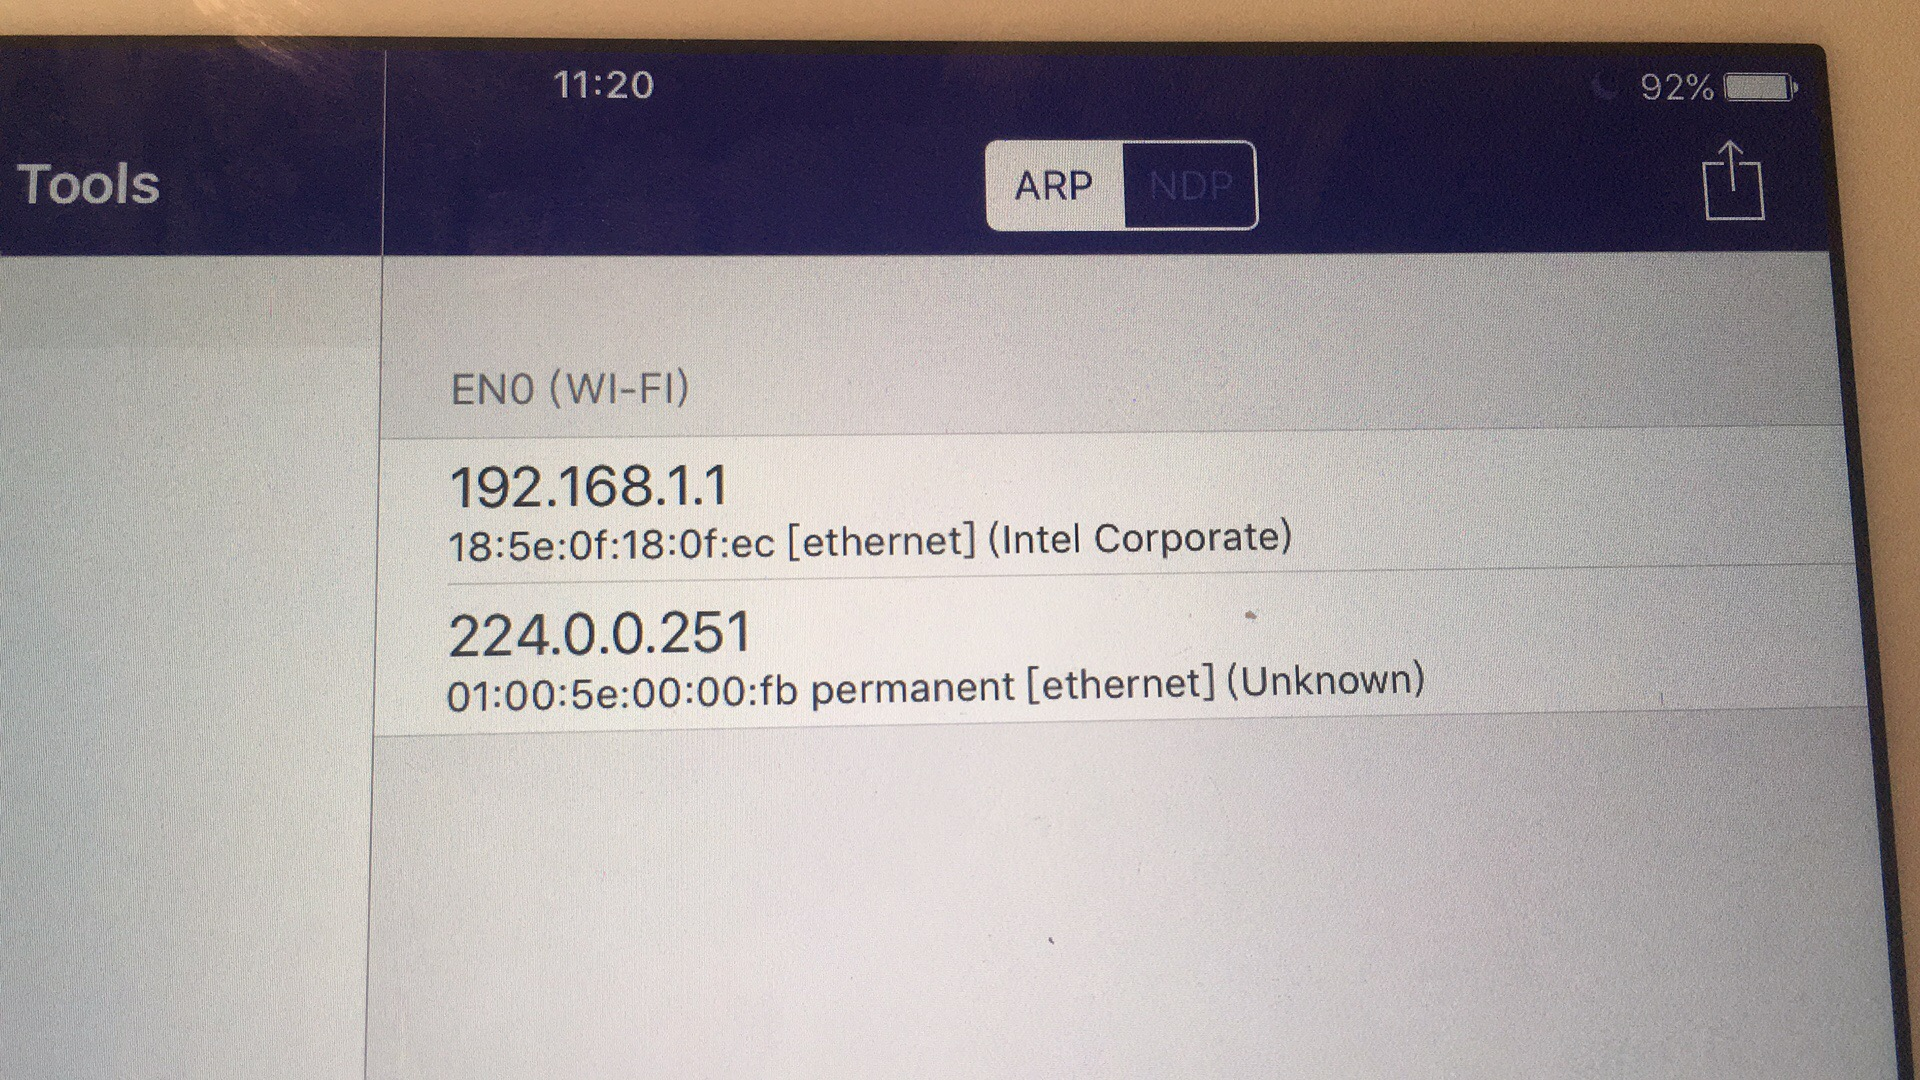
\includegraphics[width=0.9\linewidth]{ipad_arp.jpg}
\caption{iPad上的arp缓存}
\label{fig:ipad_arp}
\end{figure}

图\ref{fig:wifi_arp}和图\ref{fig:ipad_arp}显示了路由器和iPad上的arp缓存,显示的MAC地址均为攻击者设备的MAC地址。

\begin{figure}[htp]
\centering
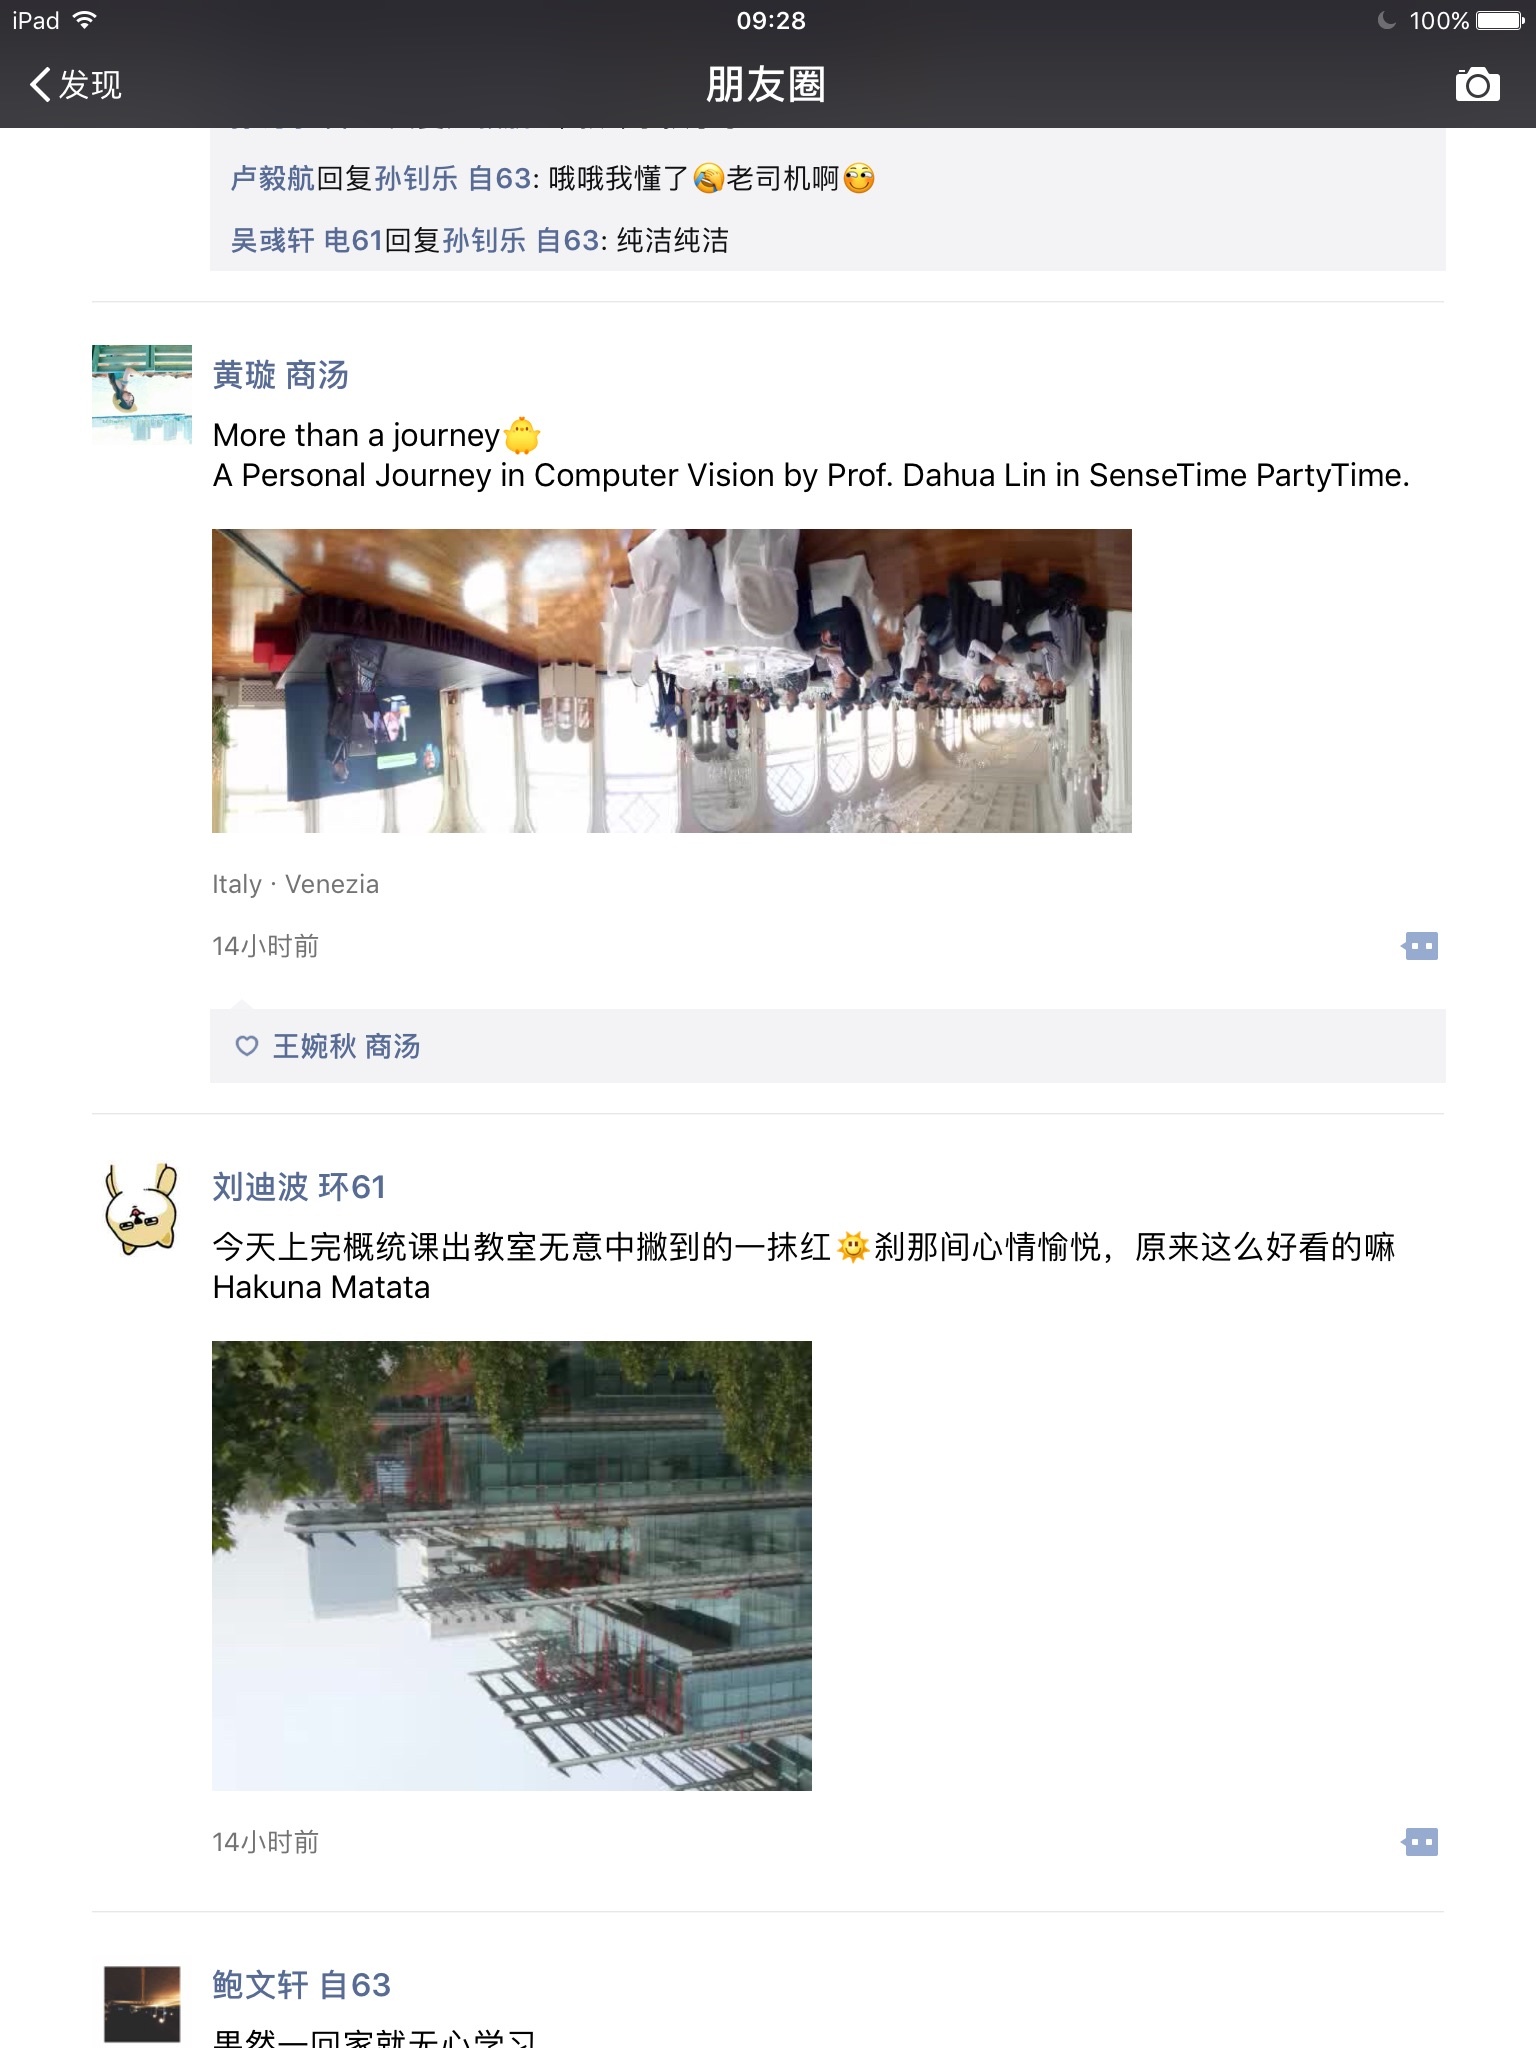
\includegraphics[width=0.6\linewidth]{ipad_wx.jpg}
\caption{查看微信朋友圈中的图片}
\label{fig:ipad_wx}
\end{figure}

图\ref{fig:ipad_wx}显示了在iPad上查看微信朋友圈图片的截图,可见微信的朋友圈的图片传输使用http协议。但是如果在群聊中发图片,发现不能被倒置,可能原因是这些图片传输走的是微信自己的协议。

\begin{figure}[htp]
\centering
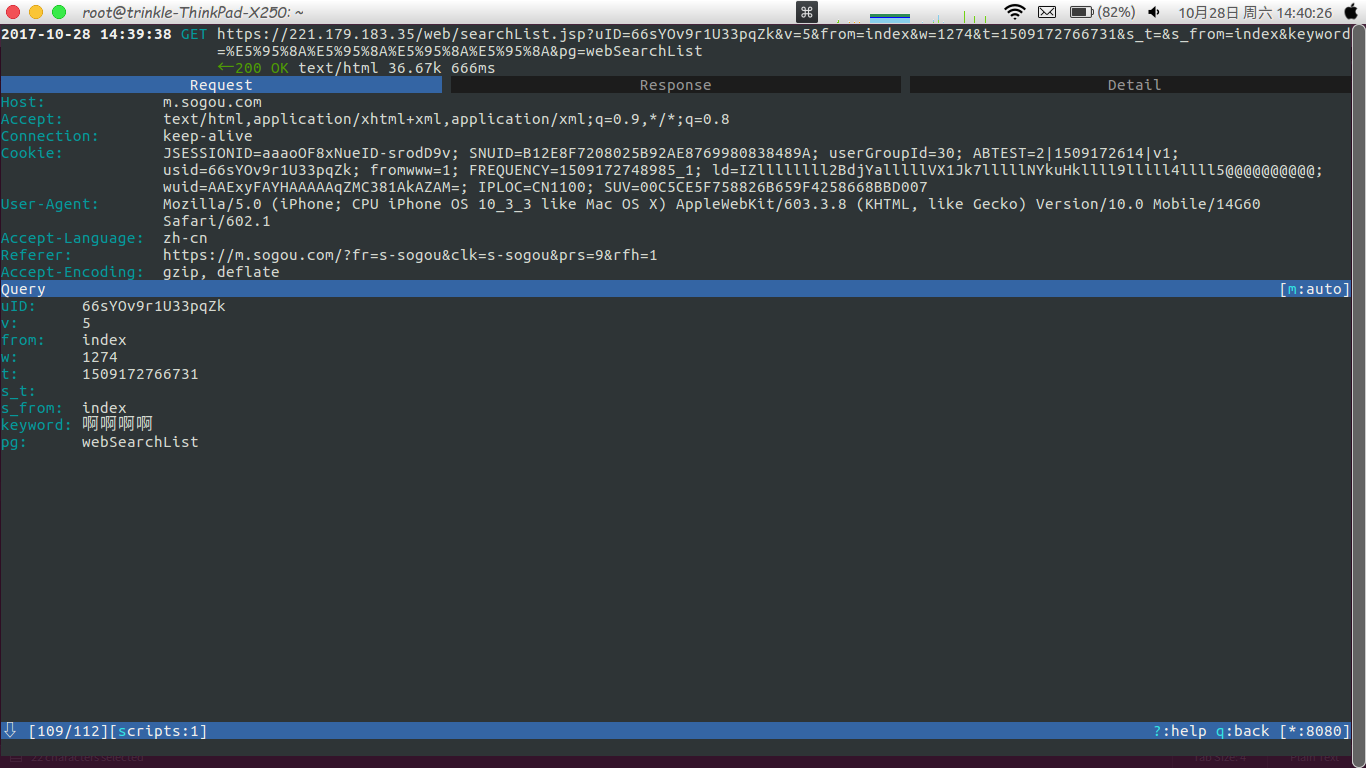
\includegraphics[width=0.9\linewidth]{se_sogou.png}
\caption{在iPhone上使用搜狗搜索}
\label{fig:se_sogou}
\end{figure}

图\ref{fig:se_sogou}显示了在iPhone上使用搜狗搜索,在攻击者机器上看到的报文信息。同之前Win10一样,会出来一个提示框,说链接不安全/证书有问题,然后一旦点击继续,流量就会被中间人截获,比如图\ref{fig:se_wlxt}所示,网络学堂的帐号密码直接被窃听。

\begin{figure}[htp]
\centering
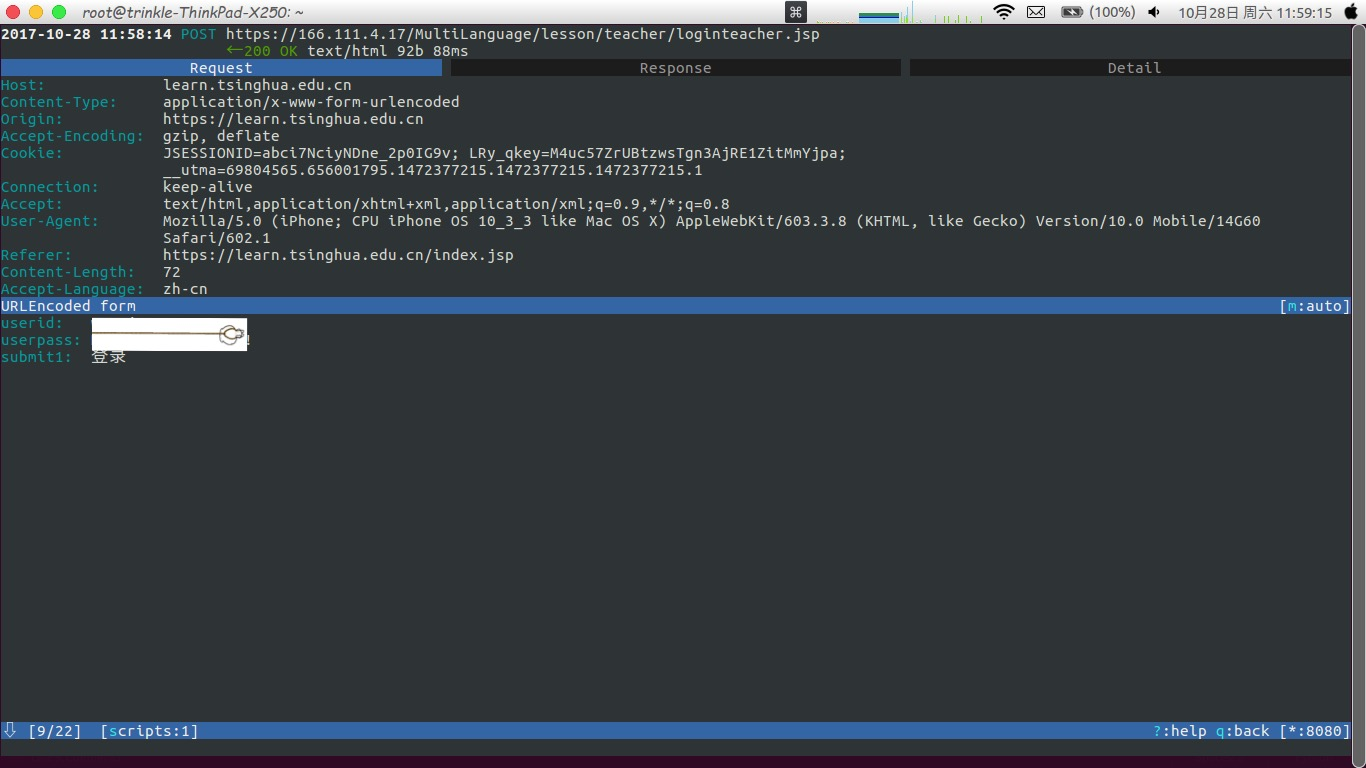
\includegraphics[width=0.9\linewidth]{se_wlxt.jpg}
\caption{在iPhone上登录网页版网络学堂}
\label{fig:se_wlxt}
\end{figure}

\subsection{小米手机}
配置与之前相同。发现无法被欺骗,并且无法上网。考虑到之前Macbook Pro上的现象,只好手动将手机连接的wifi的代理手动设置为攻击者的ip地址和8080端口,发现能够被欺骗。

测试了一下AtTsinghua,发现一部分的密码使用MD5进行传输,另一部分使用明文传输,可见AtTsinghua也并不安全。

\subsection{攻击者为Ubuntu虚拟机}
配置与之前相同。靶机为原来的攻击者。虚拟机网络设置为VirtualBox中的“桥接网卡-全部允许”选项。发现欺骗不成功。

查看arp缓存,发现arp的包发送出去了,但是MAC地址为虚拟机所在的Win10的MAC地址。我们尝试过手动修改arp的hwsrc参数,可是仍然无济于事。猜想:在arp包发送出去的时候,Win10自动转发,并且写上自己的MAC地址。于是双方arp的缓存被改为了Win10的MAC地址,所有的流量都到了Windows上,无法被Ubuntu虚拟机所监听。
\end{document}
